\chapter{Sample game}

We provide a very simple sample game so everyone can see how it works. 

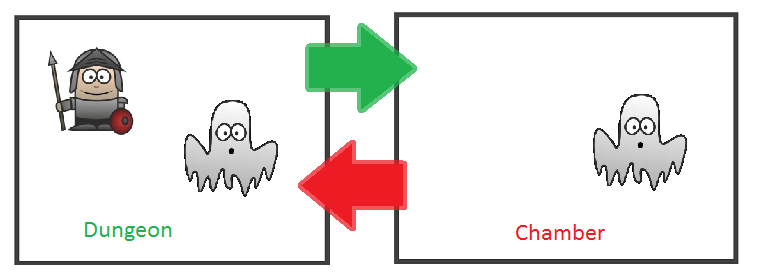
\includegraphics[scale=0.75]{assets/SampleGame.png}
 The sample game consists of 2 Rooms which are connected to each other. Each room has one "Ghost" creature and the first room also contains the player and an "Apple" item.  The player also has some items in his inventory.
 
 An example for a creature or player:
 \begin{verbatim}
 <player name="Mike Moore" life="100" xcordinate="1" ycordinate="1">
        <item ref="knife" />
        <item ref="lamp" />
        <item ref="apple" />
    </player>
 \end{verbatim}
 The  attributes name,life and x,y-cordinates to determine the status and stats of the player.
 The item elements are then used to specify which items the player has in his inventory.
 
 The items are basicly just a bunch off attributes and there really easy to create :
 \begin{verbatim}
 <equip-item
        id="knife"
        name="Knife"
        description="A sharp knife, use with caution!"
        damage="5" />
 \end{verbatim}
All item have a id,name and description, equip items also can have additional stats.

The full xml file can be found in the appendix or at \href{https://github.com/kerko/epic/blob/dev/project/demo/demo.xml}{GitHub}